\documentclass{article}
\usepackage[utf8]{inputenc}
\usepackage[french]{babel}
\usepackage[T1]{fontenc}
\usepackage{algorithm}
\usepackage{graphicx}
\usepackage{float}

\title{}
\author{}
\date{}


\setlength{\parindent}{0cm}
\setlength{\parskip}{1ex plus 0.5ex minus 0.2ex}
\newcommand{\hsp}{\hspace{20pt}}
\newcommand{\HRule}{\rule{\linewidth}{0.5mm}}


\title{}
\author{}
\date{}

\makeatletter
\def\BState{\State\hskip-\ALG@thistlm}
\makeatother


\begin{document}

\begin{titlepage}
  \begin{sffamily}
  \begin{center}

    % Upper part of the page. The '~' is needed because \\
    % only works if a paragraph has started.

    \textsc{\LARGE Polytech Sorbonne}\\[2cm]

    \textsc{\Large EPU-N7-IOB}\\[1.5cm]

    % Title
    \HRule \\[0.4cm]
    { \huge \bfseries FFT et arithmétique rapide\\[0.4cm] }

    \HRule \\[2cm]
    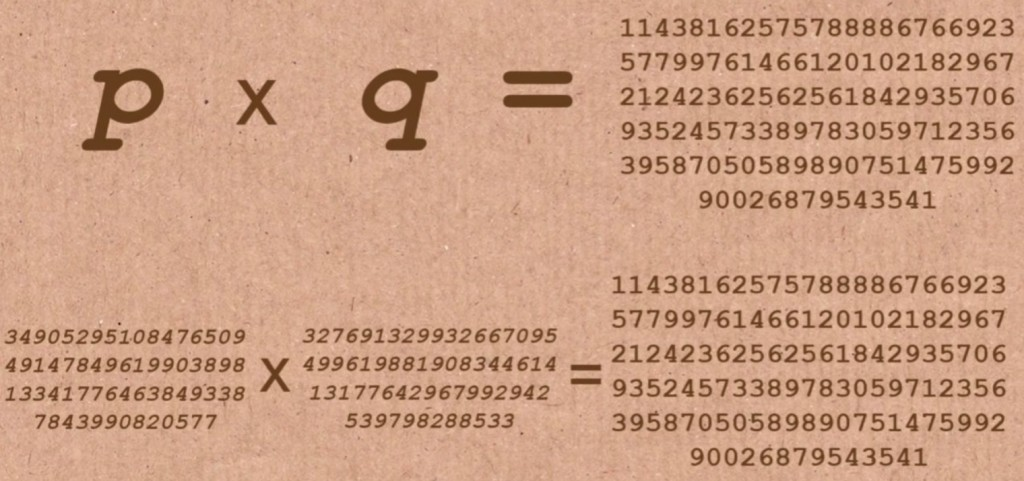
\includegraphics[scale=0.35]{assets/img/rsa.jpeg}
    \\[2cm]

    \vfill
    \begin{minipage}{0.4\textwidth}
      \begin{center} \large
        Arthur Guillec\\
      \end{center}
    \end{minipage}
    \vfill

  \end{center}
  \end{sffamily}
\end{titlepage}


\section{Introduction}

\section{Test}

\section{Conclusion}

\end{document}